\documentclass{../TexTemplate/myslide}
\usepackage[slide,table,python]{../TexTemplate/mypackage}
\hypersetup{colorlinks=true,linkcolor=black,urlcolor=blue}
\usepackage{xcolor}

\renewcommand{\thefootnote}{\fnsymbol{footnote}}

\title[ToolsSeminar]{Tools Seminar}
\subtitle{Week 7 - Machine Learning}
\author[chhzh123]{Hongzheng~Chen}
\date[Mar 9, 2020]{Mar 9, 2020}

\begin{document}

\begin{frame}
\titlepage
\end{frame}

\begin{frame}
\tableofcontents
\end{frame}

\section{Introduction}
\begin{frame}
\sectionpage
\end{frame}

\begin{frame}{Machine Learning}
\begin{quote}
A computer program is said to learn from experience $E$ with respect to some class of tasks $T$ and performance measure $P$,
if its performance at tasks in $T$, as measured by $P$, improves with experience $E$.\\
\hfill--- Mitchell, 1997
% 每个机器学习都可以被精准地定义为:1) 任务T;2) 训练过程E;3) 模型表现P。
% 而学习过程则可以被拆解为「为了实现任务T」,我们「通过训练过程E」,逐步「提高表现P」的一个过程。
\end{quote}
\bigskip
Take exam as an example
\begin{itemize}
	\item $T$: To obtain high score
	\item $E$: Do exercise
	\item $P$: Accuracy of exercise
\end{itemize}
\end{frame}

\begin{frame}{Machine Learning Branches}
\begin{figure}[H]
\centering
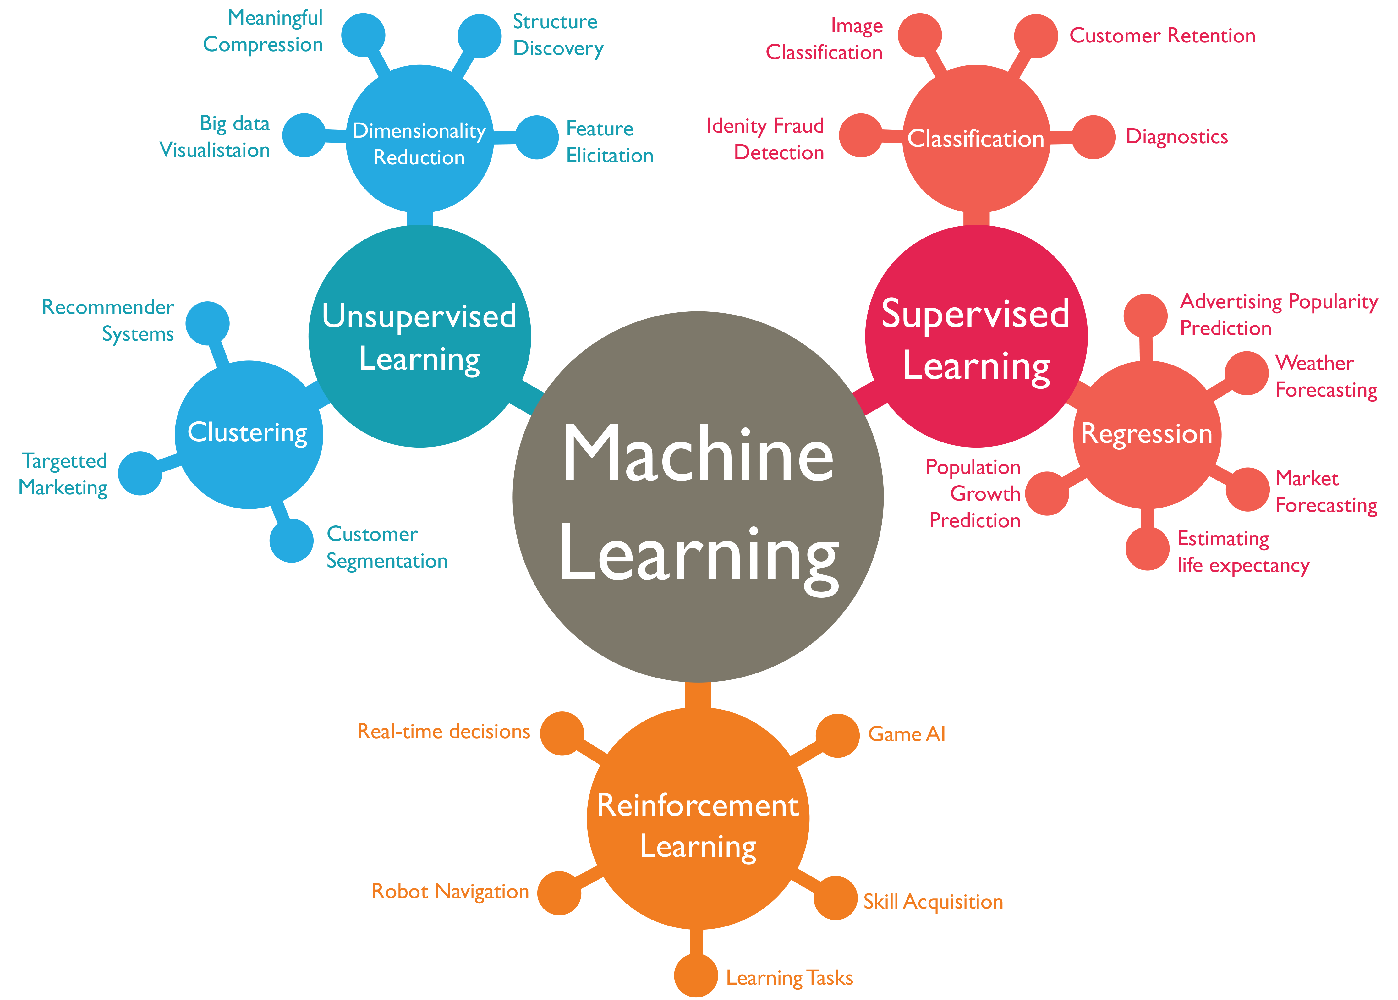
\includegraphics[width=0.8\linewidth]{fig/ml_branches.png}
\caption*{\small Fig source: \url{https://askdatascience.com/13/what-are-the-main-branches-of-machine-learning}}
\end{figure}
\end{frame}

\begin{frame}{Some Ideas to Clarify}
\begin{center}
\textbf{Artificial Intelligence (AI)\\
\qquad $>$ Machine Learning (ML)\\
\qquad\qquad $>$ Deep Learning (DL)}
\end{center}
\begin{itemize}
	\item ML is not the only way to achieve AI
	\item DL is just a method of ML
	\item Neural Network (NN) is the core of DL
	\item Computer Vision (CV) \& Natural Language Processing (NLP) are two applications of DL
\end{itemize}
\end{frame}

\section{Some Introductory Books \& Courses}
\begin{frame}
\sectionpage
\end{frame}

\begin{frame}{Machine Learning}
Prerequirement: \href{http://cs229.stanford.edu/section/cs229-linalg.pdf}{Linear algebra}, multivariable calculus, \href{http://cs229.stanford.edu/section/cs229-prob.pdf}{probability theory}
\begin{itemize}
	\item Andrew Ng, \href{http://cs229.stanford.edu/}{Stanford CS229: Machine Learning}
	\item Hsuan-Tien Lin, \href{https://www.csie.ntu.edu.tw/~htlin/course/mlfound19fall/}{NTU: Machine Learning Foundations}
\end{itemize}
You can find them on Bilibili!\\\bigskip
% 如何用3个月零基础入门「机器学习」? - 微调的文章 - 知乎
% https://zhuanlan.zhihu.com/p/29704017
* YJango, \href{https://space.bilibili.com/344849038/channel/detail?cid=54015}{《学习观》}
\end{frame}

\begin{frame}{Chinese Books}
\begin{figure}
\centering
\begin{tabular}{ccc}
\href{https://book.douban.com/subject/26708119/}{
\includegraphics[width=0.3\linewidth]{fig/watermelon_book.jpg}} &
\href{https://item.jd.com/47384022706.html}{
\includegraphics[width=0.32\linewidth]{fig/statistical_ml.jpg}}&
\href{https://book.douban.com/subject/24703171/}{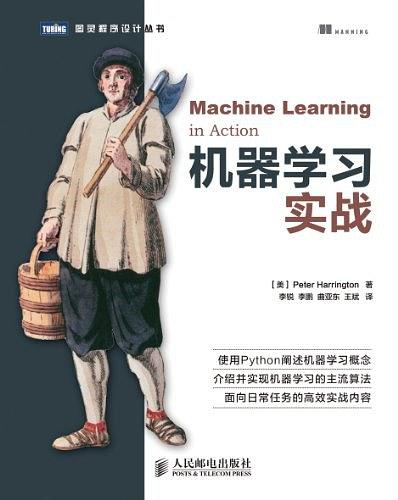
\includegraphics[width=0.25\linewidth]{fig/ml_in_action.jpg}}
\end{tabular}
\end{figure}
\end{frame}

\begin{frame}{Other books}
\begin{itemize}
	\item Christopher M. Bishop, \href{http://users.isr.ist.utl.pt/~wurmd/Livros/school/Bishop\%20-\%20Pattern\%20Recognition\%20And\%20Machine\%20Learning\%20-\%20Springer\%20\%202006.pdf}{Pattern Recognition \& Machine Learning (PRML)}
	\item Stephen Boyd, Lieven Vandenberghe, \href{https://web.stanford.edu/~boyd/cvxbook/bv_cvxbook.pdf}{Convex Optimization}
	\item Ian Goodfellow, Yoshua Bengio, Aaron Courville, \href{https://www.deeplearningbook.org/}{Deep Learning} (flower book)
	\item Richard S. Sutton, Andrew G. Barto, \href{https://web.stanford.edu/class/psych209/Readings/SuttonBartoIPRLBook2ndEd.pdf}{Reinforcement Learning}
\end{itemize}
\end{frame}

\begin{frame}{Top-tier Conferences in AI Area}
\begin{itemize}
	\item General AI: \underline{AAAI}, \underline{IJCAI}
	\item NLP: \underline{ACL}, EMNLP, NAACL
	\item CV: \underline{CVPR}, \underline{ICCV}, ECCV
	\item ML: \underline{NeurIPS/NIPS}, \underline{ICML}, ICLR
	\item Data mining: \underline{KDD}, \underline{SIGMOD}, \underline{ICDE}, \underline{VLDB}, \underline{SIGIR}, \underline{WWW}
	\item System: SysML
\end{itemize}
\end{frame}

\section{Machine Learning Basis}
\begin{frame}
\sectionpage
\end{frame}

\begin{frame}{Machine Learning Basis}
For \textbf{supervised learning} (classification \& regression), we have
\begin{itemize}
	\item Training set
	\[\mathcal{D}=\{(\vx_1,y_1),(\vx_2,y_2),\ldots,(\vx_m,y_m)\}\]
	\begin{itemize}
		\item Sample: $(\vx_i,y_i)$
		\item Input/Feature/Attribute: $\vx_i\in\mathcal{X}\subset\rr^d$
		\item Output/Label/Target: $y_i\in\mathcal{Y}\subset\rr$
	\end{itemize}
	\item Model: Want to learn a mapping from $\mathcal{X}$ to $\mathcal{Y}$
	\[f:\mathcal{X}\mapsto\mathcal{Y}\]
\end{itemize}
For example, consider face recognition
\begin{itemize}
	\item Input: Many students' faces in 2D figures
% Commonly, for figures, we have 4D tensor
% \[sample \times channel \times x \times y\]
	\item Output: The name of the student
	\item Model: $f(\text{face})=\text{student}$
\end{itemize}
Differences between different ML alg. are how to determine $f$
\end{frame}

\begin{frame}{Linear Regression}
Consider sample with $d$ features
\[\vx=(x_1,x_2,\ldots,x_d)\]
Use \textbf{linear combination} of features as model
\[f(\vx)=w_1x_1+w_2x_2+\cdots+w_dx_d+b=\vw^\T\vx+b\simeq y\]
where $\vw$, $b$ are the parameter needs to be learned\\
\textbf{Loss function} $J(\vw,b)$: measure the performance of the model, we use \textbf{mean square error (MSE)} here
\[J(\vw,b) = \norm{f(\vx_i)-y_i}_2^2\]
Then \textbf{objective} is to optimize
\[\min_{\vw,b} \lrp{\sum_{i=1}^m J(\vw,b)} = \min_{\vw,b} \lrp{\sum_{i=1}^m \norm{f(\vx_i)-y_i}_2^2}\]
\end{frame}

\begin{frame}{Linear Regression}
The best parameters are what we want
\[(\vw^*,b^*)=\argmin_{\vw,b}\lrp{\sum_{i=1}^m \norm{f(\vx_i)-y_i}_2^2}\]
Commonly, we use \href{https://xavierbourretsicotte.github.io/animation_ridge.html}{gradient descent} to optimize, which is an iterative process
\[\begin{cases}
\vw^{(k+1)} = \vw^{(k)} - \alpha\frac{\partial J(\vw,b)}{\partial \vw} &= \vw^{(k)} - \alpha\nabla_{\vw}{J(\vw,b)}\\
b^{(k+1)} = b^{(k)} - \alpha\frac{\partial J(\vw,b)}{\partial b} &= b^{(k)} - \alpha\nabla_{b}{J(\vw,b)}
\end{cases}\]
If loss cannot be reduced more (converged), we find the optimal $\vw^*$ and $b^*$\\
The final model becomes
\[f(\vx)=(\vw^*)^\T\vx+b^*\]
\end{frame}

\begin{frame}{Linear Regression}
But for MSE of linear regression, you can easily find close-form solution by \textbf{least square method}
\begin{itemize}
	\item Stack the samples
	\[X=\bmat{x_{11} & x_{12} & \cdots & x_{1d} & 1\\
	x_{21} & x_{22} & \cdots & x_{2d} & 1\\
	\vdots & \vdots & \ddots & \vdots & \vdots\\
	x_{m1} & x_{m2} & \cdots & x_{md} & 1}=
	\bmat{\vx_1^\T & 1\\
	\vx_2^\T & 1\\
	\vdots & \vdots\\
	\vx_m^\T & 1},\;
	\vy=\bmat{y_1\\y_2\\\vdots\\ y_m},\;
	\hat{\vw}=\bmat{w_1\\\vdots\\ w_d\\b}\]
	\item Optimize
	\[\hat{\vw}^*={\arg\min}_{\hat{\vw}}\;(\vy-X\hat{\vw})^\T(\vy-X\hat{\vw})\]
	\item Make derivative as $0$
	\[\pd{J(\hat{\vw})}{\hat{\vw}}=2X^\T(X\hat{\vw}-\vy)=0\]
	\item Solve for best $\hat{\vw}$ (if $X^\T X$ has inverse)
	\[\hat{\vw}^*=(X^\T X)^{-1}X^\T\vy\]
\end{itemize}
\end{frame}

\begin{frame}{Summary}
\begin{enumerate}
	\item Obtain required training and testing data
	\item Determine the objective of the task
	\item Select a machine learning model to train
	\item Use pre-trained model to predict
\end{enumerate}
\end{frame}

\section{Data Processing}
\begin{frame}
\sectionpage
\end{frame}

\begin{frame}{Machine Learning Today}
\begin{figure}
\centering
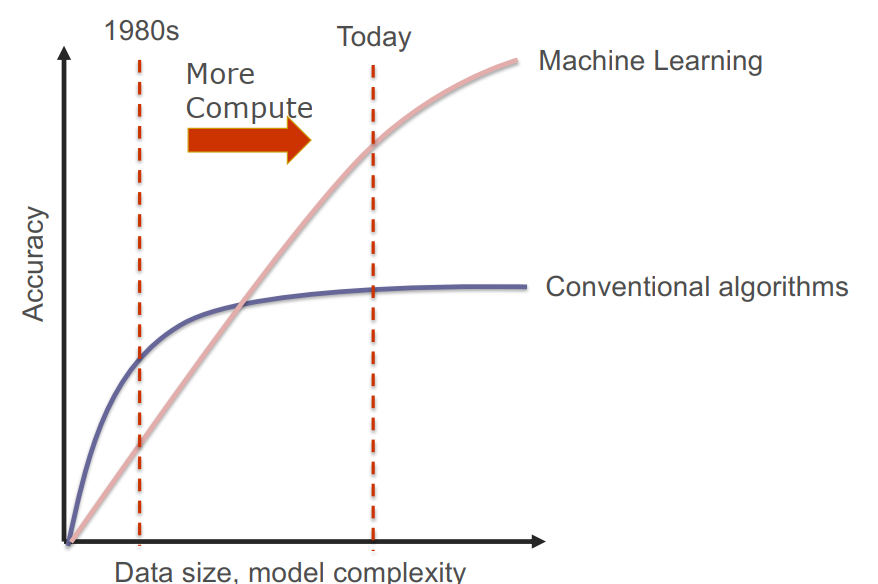
\includegraphics[width=0.8\linewidth]{fig/ml_today.png}
\caption*{\small Fig source: Jeff Dean, HotChips 2017}
\end{figure}
\end{frame}

\begin{frame}{Software 2.0 Era}
Training data: The new input to software 2.0
\begin{figure}
\centering
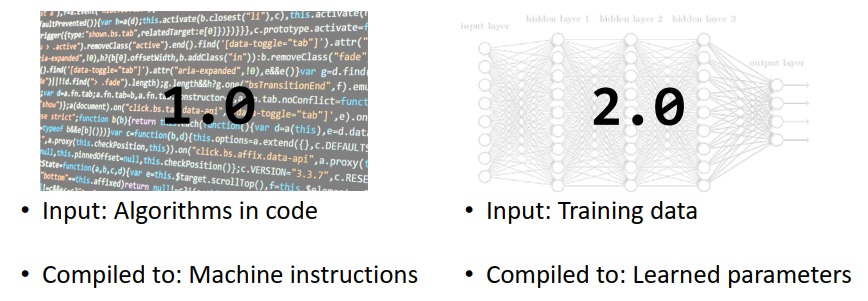
\includegraphics[width=0.9\linewidth]{fig/software2.png}
\caption*{\small Fig source: Kunle Olukutun, ISCA, 2018}
\end{figure}
Thus, \textbf{quality \& quantity} of the data determine performance!
\end{frame}

\begin{frame}{Common Data Science Steps}
\begin{enumerate}
	\item Data collection
	\item Feature engineering (Data cleaning/preprocessing)
	\item Model selection
	\item Training
	\item Evaluation
\end{enumerate}
\end{frame}

\begin{frame}[fragile]{Data Collection}
In competitions, we commonly have official datasets\\
But what if no collected datasets available in some specific tasks?\\
(e.g. face mask recognition)\\
\pause
\textbf{Design a web crawler!}
\begin{enumerate}
	\item Crawl the webpages (\verb'requests', \verb'urllib')
	\item Parse html (\verb'bs4')
	\item Retrieve useful data (text, figure, or other specific content)
	\item Organize the data
	\item Store them into files (\verb'mysql', \verb'json')
\end{enumerate}
\end{frame}

\begin{frame}{A Dataset Example}
\begin{center}
\begin{tabular}{cccccc}\hline
 & Feat 1 & Feat 2 & $\cdots$ & Feat $d$ & Label\\\hline
Sample 1 & $x_{11}$ & $x_{12}$ & & & $y_1$ \\\hline
$\vdots$ & & & & & $\vdots$\\\hline
Sample $m$ & & & & & $y_m$ \\\hline
\end{tabular}
\end{center}
\end{frame}

\begin{frame}{Data Cleaning}
Data cleaning or feature engineering is \textbf{the first step} of most ML tasks!\\
Most datasets are troublesome: (think about questionnaires)
% 特征工程到底是什么? - 城东的回答 - 知乎
% https://www.zhihu.com/question/29316149/answer/110159647
\begin{itemize}
	\item Data missing
	\item Redundant data
	\item Data not in same scale
	\item Useless features
	\item Too many features
	\item $\cdots$
\end{itemize}
ML is also called \textbf{representative learning}\\
Good data and good features benefit learning process
\end{frame}

\section{Pandas \& Sklearn}
\begin{frame}
\sectionpage
\end{frame}

\begin{frame}{Some Hints}
Use jupyter notebook for interactive operations, see demo
\begin{itemize}
	\item You should carefully deal with the data which may be very dirty
	\item For models with hyperparameters, use \href{https://scikit-learn.org/stable/modules/grid_search.html}{grid search} to fine-tune
\end{itemize}
\end{frame}

\section{Summary}
\begin{frame}
\sectionpage
\end{frame}

\begin{frame}{Summary}
\begin{itemize}
	\item Introduction
	\item Machine learning basis: Linear regression
	\item Data processing: pandas
	\item Training \& Testing: sklearn
\end{itemize}
\end{frame}

\end{document}